
%% bare_conf.tex
%% V1.3
%% 2007/01/11
%% by Michael Shell
%% See:
%% http://www.michaelshell.org/
%% for current contact information.
%%
%% This is a skeleton file demonstrating the use of IEEEtran.cls
%% (requires IEEEtran.cls version 1.7 or later) with an IEEE conference paper.
%%
%% Support sites:
%% http://www.michaelshell.org/tex/ieeetran/
%% http://www.ctan.org/tex-archive/macros/latex/contrib/IEEEtran/
%% and
%% http://www.ieee.org/

%%*************************************************************************
%% Legal Notice:
%% This code is offered as-is without any warranty either expressed or
%% implied; without even the implied warranty of MERCHANTABILITY or
%% FITNESS FOR A PARTICULAR PURPOSE!
%% User assumes all risk.
%% In no event shall IEEE or any contributor to this code be liable for
%% any damages or losses, including, but not limited to, incidental,
%% consequential, or any other damages, resulting from the use or misuse
%% of any information contained here.
%%
%% All comments are the opinions of their respective authors and are not
%% necessarily endorsed by the IEEE.
%%
%% This work is distributed under the LaTeX Project Public License (LPPL)
%% ( http://www.latex-project.org/ ) version 1.3, and may be freely used,
%% distributed and modified. A copy of the LPPL, version 1.3, is included
%% in the base LaTeX documentation of all distributions of LaTeX released
%% 2003/12/01 or later.
%% Retain all contribution notices and credits.
%% ** Modified files should be clearly indicated as such, including  **
%% ** renaming them and changing author support contact information. **
%%
%% File list of work: IEEEtran.cls, IEEEtran_HOWTO.pdf, bare_adv.tex,
%%                    bare_conf.tex, bare_jrnl.tex, bare_jrnl_compsoc.tex
%%*************************************************************************

% *** Authors should verify (and, if needed, correct) their LaTeX system  ***
% *** with the testflow diagnostic prior to trusting their LaTeX platform ***
% *** with production work. IEEE's font choices can trigger bugs that do  ***
% *** not appear when using other class files.                            ***
% The testflow support page is at:
% http://www.michaelshell.org/tex/testflow/



% Note that the a4paper option is mainly intended so that authors in
% countries using A4 can easily print to A4 and see how their papers will
% look in print - the typesetting of the document will not typically be
% affected with changes in paper size (but the bottom and side margins will).
% Use the testflow package mentioned above to verify correct handling of
% both paper sizes by the user's LaTeX system.
%
% Also note that the "draftcls" or "draftclsnofoot", not "draft", option
% should be used if it is desired that the figures are to be displayed in
% draft mode.
%
\documentclass[conference]{IEEEtran}
% Add the compsoc option for Computer Society conferences.
%
% If IEEEtran.cls has not been installed into the LaTeX system files,
% manually specify the path to it like:
% \documentclass[conference]{../sty/IEEEtran}

\usepackage{times,amsmath,epsfig}
\usepackage[linesnumbered,ruled]{algorithm2e}

%\usepackage[pdftex]{graphicx}
% For figures
\usepackage{graphicx} % more modern
\usepackage{epsfig} % less modern
\usepackage{subfigure}
\usepackage{enumerate}
%\usepackage[pdftex]{graphicx}
% For figures
\usepackage{graphicx} % more modern
%\usepackage{epsfig} % less modern
\usepackage{subfigure}

\usepackage{mathrsfs}
\usepackage{amsmath}



% Some very useful LaTeX packages include:
% (uncomment the ones you want to load)


% *** MISC UTILITY PACKAGES ***
%
%\usepackage{ifpdf}
% Heiko Oberdiek's ifpdf.sty is very useful if you need conditional
% compilation based on whether the output is pdf or dvi.
% usage:
% \ifpdf
%   % pdf code
% \else
%   % dvi code
% \fi
% The latest version of ifpdf.sty can be obtained from:
% http://www.ctan.org/tex-archive/macros/latex/contrib/oberdiek/
% Also, note that IEEEtran.cls V1.7 and later provides a builtin
% \ifCLASSINFOpdf conditional that works the same way.
% When switching from latex to pdflatex and vice-versa, the compiler may
% have to be run twice to clear warning/error messages.






% *** CITATION PACKAGES ***
%
%\usepackage{cite}
% cite.sty was written by Donald Arseneau
% V1.6 and later of IEEEtran pre-defines the format of the cite.sty package
% \cite{} output to follow that of IEEE. Loading the cite package will
% result in citation numbers being automatically sorted and properly
% "compressed/ranged". e.g., [1], [9], [2], [7], [5], [6] without using
% cite.sty will become [1], [2], [5]--[7], [9] using cite.sty. cite.sty's
% \cite will automatically add leading space, if needed. Use cite.sty's
% noadjust option (cite.sty V3.8 and later) if you want to turn this off.
% cite.sty is already installed on most LaTeX systems. Be sure and use
% version 4.0 (2003-05-27) and later if using hyperref.sty. cite.sty does
% not currently provide for hyperlinked citations.
% The latest version can be obtained at:
% http://www.ctan.org/tex-archive/macros/latex/contrib/cite/
% The documentation is contained in the cite.sty file itself.






% *** GRAPHICS RELATED PACKAGES ***
%
\ifCLASSINFOpdf
  % \usepackage[pdftex]{graphicx}
  % declare the path(s) where your graphic files are
  % \graphicspath{{../pdf/}{../jpeg/}}
  % and their extensions so you won't have to specify these with
  % every instance of \includegraphics
  % \DeclareGraphicsExtensions{.pdf,.jpeg,.png}
\else
  % or other class option (dvipsone, dvipdf, if not using dvips). graphicx
  % will default to the driver specified in the system graphics.cfg if no
  % driver is specified.
  % \usepackage[dvips]{graphicx}
  % declare the path(s) where your graphic files are
  % \graphicspath{{../eps/}}
  % and their extensions so you won't have to specify these with
  % every instance of \includegraphics
  % \DeclareGraphicsExtensions{.eps}
\fi
% graphicx was written by David Carlisle and Sebastian Rahtz. It is
% required if you want graphics, photos, etc. graphicx.sty is already
% installed on most LaTeX systems. The latest version and documentation can
% be obtained at:
% http://www.ctan.org/tex-archive/macros/latex/required/graphics/
% Another good source of documentation is "Using Imported Graphics in
% LaTeX2e" by Keith Reckdahl which can be found as epslatex.ps or
% epslatex.pdf at: http://www.ctan.org/tex-archive/info/
%
% latex, and pdflatex in dvi mode, support graphics in encapsulated
% postscript (.eps) format. pdflatex in pdf mode supports graphics
% in .pdf, .jpeg, .png and .mps (metapost) formats. Users should ensure
% that all non-photo figures use a vector format (.eps, .pdf, .mps) and
% not a bitmapped formats (.jpeg, .png). IEEE frowns on bitmapped formats
% which can result in "jaggedy"/blurry rendering of lines and letters as
% well as large increases in file sizes.
%
% You can find documentation about the pdfTeX application at:
% http://www.tug.org/applications/pdftex





% *** MATH PACKAGES ***
%
%\usepackage[cmex10]{amsmath}
% A popular package from the American Mathematical Society that provides
% many useful and powerful commands for dealing with mathematics. If using
% it, be sure to load this package with the cmex10 option to ensure that
% only type 1 fonts will utilized at all point sizes. Without this option,
% it is possible that some math symbols, particularly those within
% footnotes, will be rendered in bitmap form which will result in a
% document that can not be IEEE Xplore compliant!
%
% Also, note that the amsmath package sets \interdisplaylinepenalty to 10000
% thus preventing page breaks from occurring within multiline equations. Use:
%\interdisplaylinepenalty=2500
% after loading amsmath to restore such page breaks as IEEEtran.cls normally
% does. amsmath.sty is already installed on most LaTeX systems. The latest
% version and documentation can be obtained at:
% http://www.ctan.org/tex-archive/macros/latex/required/amslatex/math/





% *** SPECIALIZED LIST PACKAGES ***
%
%\usepackage{algorithmic}
% algorithmic.sty was written by Peter Williams and Rogerio Brito.
% This package provides an algorithmic environment fo describing algorithms.
% You can use the algorithmic environment in-text or within a figure
% environment to provide for a floating algorithm. Do NOT use the algorithm
% floating environment provided by algorithm.sty (by the same authors) or
% algorithm2e.sty (by Christophe Fiorio) as IEEE does not use dedicated
% algorithm float types and packages that provide these will not provide
% correct IEEE style captions. The latest version and documentation of
% algorithmic.sty can be obtained at:
% http://www.ctan.org/tex-archive/macros/latex/contrib/algorithms/
% There is also a support site at:
% http://algorithms.berlios.de/index.html
% Also of interest may be the (relatively newer and more customizable)
% algorithmicx.sty package by Szasz Janos:
% http://www.ctan.org/tex-archive/macros/latex/contrib/algorithmicx/




% *** ALIGNMENT PACKAGES ***
%
%\usepackage{array}
% Frank Mittelbach's and David Carlisle's array.sty patches and improves
% the standard LaTeX2e array and tabular environments to provide better
% appearance and additional user controls. As the default LaTeX2e table
% generation code is lacking to the point of almost being broken with
% respect to the quality of the end results, all users are strongly
% advised to use an enhanced (at the very least that provided by array.sty)
% set of table tools. array.sty is already installed on most systems. The
% latest version and documentation can be obtained at:
% http://www.ctan.org/tex-archive/macros/latex/required/tools/


%\usepackage{mdwmath}
%\usepackage{mdwtab}
% Also highly recommended is Mark Wooding's extremely powerful MDW tools,
% especially mdwmath.sty and mdwtab.sty which are used to format equations
% and tables, respectively. The MDWtools set is already installed on most
% LaTeX systems. The lastest version and documentation is available at:
% http://www.ctan.org/tex-archive/macros/latex/contrib/mdwtools/


% IEEEtran contains the IEEEeqnarray family of commands that can be used to
% generate multiline equations as well as matrices, tables, etc., of high
% quality.


%\usepackage{eqparbox}
% Also of notable interest is Scott Pakin's eqparbox package for creating
% (automatically sized) equal width boxes - aka "natural width parboxes".
% Available at:
% http://www.ctan.org/tex-archive/macros/latex/contrib/eqparbox/





% *** SUBFIGURE PACKAGES ***
%\usepackage[tight,footnotesize]{subfigure}
% subfigure.sty was written by Steven Douglas Cochran. This package makes it
% easy to put subfigures in your figures. e.g., "Figure 1a and 1b". For IEEE
% work, it is a good idea to load it with the tight package option to reduce
% the amount of white space around the subfigures. subfigure.sty is already
% installed on most LaTeX systems. The latest version and documentation can
% be obtained at:
% http://www.ctan.org/tex-archive/obsolete/macros/latex/contrib/subfigure/
% subfigure.sty has been superceeded by subfig.sty.



%\usepackage[caption=false]{caption}
%\usepackage[font=footnotesize]{subfig}
% subfig.sty, also written by Steven Douglas Cochran, is the modern
% replacement for subfigure.sty. However, subfig.sty requires and
% automatically loads Axel Sommerfeldt's caption.sty which will override
% IEEEtran.cls handling of captions and this will result in nonIEEE style
% figure/table captions. To prevent this problem, be sure and preload
% caption.sty with its "caption=false" package option. This is will preserve
% IEEEtran.cls handing of captions. Version 1.3 (2005/06/28) and later
% (recommended due to many improvements over 1.2) of subfig.sty supports
% the caption=false option directly:
%\usepackage[caption=false,font=footnotesize]{subfig}
%
% The latest version and documentation can be obtained at:
% http://www.ctan.org/tex-archive/macros/latex/contrib/subfig/
% The latest version and documentation of caption.sty can be obtained at:
% http://www.ctan.org/tex-archive/macros/latex/contrib/caption/




% *** FLOAT PACKAGES ***
%
%\usepackage{fixltx2e}
% fixltx2e, the successor to the earlier fix2col.sty, was written by
% Frank Mittelbach and David Carlisle. This package corrects a few problems
% in the LaTeX2e kernel, the most notable of which is that in current
% LaTeX2e releases, the ordering of single and double column floats is not
% guaranteed to be preserved. Thus, an unpatched LaTeX2e can allow a
% single column figure to be placed prior to an earlier double column
% figure. The latest version and documentation can be found at:
% http://www.ctan.org/tex-archive/macros/latex/base/



%\usepackage{stfloats}
% stfloats.sty was written by Sigitas Tolusis. This package gives LaTeX2e
% the ability to do double column floats at the bottom of the page as well
% as the top. (e.g., "\begin{figure*}[!b]" is not normally possible in
% LaTeX2e). It also provides a command:
%\fnbelowfloat
% to enable the placement of footnotes below bottom floats (the standard
% LaTeX2e kernel puts them above bottom floats). This is an invasive package
% which rewrites many portions of the LaTeX2e float routines. It may not work
% with other packages that modify the LaTeX2e float routines. The latest
% version and documentation can be obtained at:
% http://www.ctan.org/tex-archive/macros/latex/contrib/sttools/
% Documentation is contained in the stfloats.sty comments as well as in the
% presfull.pdf file. Do not use the stfloats baselinefloat ability as IEEE
% does not allow \baselineskip to stretch. Authors submitting work to the
% IEEE should note that IEEE rarely uses double column equations and
% that authors should try to avoid such use. Do not be tempted to use the
% cuted.sty or midfloat.sty packages (also by Sigitas Tolusis) as IEEE does
% not format its papers in such ways.





% *** PDF, URL AND HYPERLINK PACKAGES ***
%
%\usepackage{url}
% url.sty was written by Donald Arseneau. It provides better support for
% handling and breaking URLs. url.sty is already installed on most LaTeX
% systems. The latest version can be obtained at:
% http://www.ctan.org/tex-archive/macros/latex/contrib/misc/
% Read the url.sty source comments for usage information. Basically,
% \url{my_url_here}.





% *** Do not adjust lengths that control margins, column widths, etc. ***
% *** Do not use packages that alter fonts (such as pslatex).         ***
% There should be no need to do such things with IEEEtran.cls V1.6 and later.
% (Unless specifically asked to do so by the journal or conference you plan
% to submit to, of course. )


% correct bad hyphenation here
\hyphenation{op-tical net-works semi-conduc-tor}


\begin{document}
%
% paper title
% can use linebreaks \\ within to get better formatting as desired
\title{Mid-term Solar Forecast system based on Geostationary Satellite data}
% author names and affiliations
% use a multiple column layout for up to three different
% affiliations
%\author{\IEEEauthorblockN{Michael Shell}
%\IEEEauthorblockA{School of Electrical and\\Computer Engineering\\
%Georgia Institute of Technology\\
%Atlanta, Georgia 30332--0250\\
%Email: http://www.michaelshell.org/contact.html}
%\and
%\IEEEauthorblockN{Homer Simpson}
%\IEEEauthorblockA{Twentieth Century Fox\\
%Springfield, USA\\
%Email: homer@thesimpsons.com}
%\and
%\IEEEauthorblockN{James Kirk\\ and Montgomery Scott}
%\IEEEauthorblockA{Starfleet Academy\\
%San Francisco, California 96678-2391\\
%Telephone: (800) 555--1212\\
%Fax: (888) 555--1212}}
%
%% conference papers do not typically use \thanks and this command
%% is locked out in conference mode. If really needed, such as for
%% the acknowledgment of grants, issue a \IEEEoverridecommandlockouts
%% after \documentclass
%
%% for over three affiliations, or if they all won't fit within the width
%% of the page, use this alternative format:
%%
%%\author{\IEEEauthorblockN{Michael Shell\IEEEauthorrefmark{1},
%%Homer Simpson\IEEEauthorrefmark{2},
%%James Kirk\IEEEauthorrefmark{3},
%%Montgomery Scott\IEEEauthorrefmark{3} and
%%Eldon Tyrell\IEEEauthorrefmark{4}}
%%\IEEEauthorblockA{\IEEEauthorrefmark{1}School of Electrical and Computer Engineering\\
%%Georgia Institute of Technology,
%%Atlanta, Georgia 30332--0250\\ Email: see http://www.michaelshell.org/contact.html}
%%\IEEEauthorblockA{\IEEEauthorrefmark{2}Twentieth Century Fox, Springfield, USA\\
%%Email: homer@thesimpsons.com}
%%\IEEEauthorblockA{\IEEEauthorrefmark{3}Starfleet Academy, San Francisco, California 96678-2391\\
%%Telephone: (800) 555--1212, Fax: (888) 555--1212}
%%\IEEEauthorblockA{\IEEEauthorrefmark{4}Tyrell Inc., 123 Replicant Street, Los Angeles, California 90210--4321}}

\author{%
% author names are typeset in 11pt, which is the default size in the author block
{Zhenzhou Peng{\small $~^{\#1}$}, Shinjae Yoo{\small $~^{\#2}$}, Dantong
Yu{\small $~^{\#3}$}, Dong Huang{\small $~^{*4}$}}% add some space between author names and affils
\vspace{1.6mm}\\
\fontsize{10}{10}\selectfont\itshape
$~^{\#}$Stony Brook University\\
100 Nicolls Road, Stony Brook, NY 11794\\
\fontsize{9}{9}\selectfont\ttfamily\upshape
$~^{1}$zhenzhou.peng@stonybrook.edu\\


% add some space between email and affil
\vspace{1.2mm}\\
\fontsize{10}{10}\selectfont\rmfamily\itshape
$~^{*}$Brookhaven National Laboratory\\
50 Bell Avenue, Upton, NY 11973\\
\fontsize{9}{9}\selectfont\ttfamily\upshape
$~^{2}$sjyoo@bnl.gov \\
$~^{3}$dtyu@bnl.gov \\
$~^{4}$dhuang@bnl.gov \\
}
%

% use for special paper notices
%\IEEEspecialpapernotice{(Invited Paper)}
\maketitle
%
\begin{abstract}
Prediction of solar energy has become a significant concern in smart grid field.
In this paper, a mid-term forecast system is designed with utilizing Optical
Flow Motion Estimation on multi-channel geostationary data and Support Vector
Regression(SVR) on solar radiation. Different from previous
approaches, our system is trying to improve satellite model precision and fill
the gap of forecasting in 30 minutes up to 5 hours. The experiment result shows
that performance in both estimation and forecasting has been significantly
improved.
 
\end{abstract}
% IEEEtran.cls defaults to using nonbold math in the Abstract.
% This preserves the distinction between vectors and scalars. However,
% if the conference you are submitting to favors bold math in the abstract,
% then you can use LaTeX's standard command \boldmath at the very start
% of the abstract to achieve this. Many IEEE journals/conferences frown on
% math in the abstract anyway.

% no keywords




% For peer review papers, you can put extra information on the cover
% page as needed:
% \ifCLASSOPTIONpeerreview
% \begin{center} \bfseries EDICS Category: 3-BBND \end{center}
% \fi
%
% For peerreview papers, this IEEEtran command inserts a page break and
% creates the second title. It will be ignored for other modes.
% NOTE keywords are not used for conference papers so do not populate them

% \begin{keywords}
% mid-term, forecast, satellite
% \end{keywords}
%\IEEEpeerreviewmaketitle
\section{Introduction}
\label{sec:intr}


With utilization and economy concern, planning and managing of control in
advance acquires great importance in solar grids system. For the purpose of
making decisions in near future, a forecast system is needed to provide
information of solar energy tendency and distribution. In general, distribution
and variation of cloud is the main source of solar radiation fluctuation.
Therefore we propose to use Geostationary satellite data as input to extract
cloud properties and track the motion.To better understand how cloud influence
the radiation, we divide the work into two parts: Estimation of irradiance based
on current cloud information from satellite and forecast of cloud motion in near future. In short, modeling and forecasting.  

The reason of division is to improve satellite estimation model and at the same
time make robust prediction scheme. Although the idea of using satellite
data as input of solar energy estimation is not new, there are some challenging
issues on cloud related fields: 1) Cloud properties is hard to
recognize, 2) More meteorologic
variables,such as atmospheric indices are needed, 3) low Spatial and temporal
resolution of estimation.

As regards forecasting, the more uncertainties emerge with time of prediction
increases. Even in the short period of time, cloud motion is hard to detect due
to: 1) motion variation is unpredictable and hard to track,2) Cloud motion may
needs cloud classification and detection in advance, 3) formation and
deformation of cloud. Therefore the imprecision of motion estimation
will be magnified with longer time prediction. In brief, motion estimation
algorithm is required to have not only accuracy but also resolution so as to
assure the quality of prediction.



% In order to better utilize satellite data,
% we propose to use Support Vector Regression(SVR) learning strategy on
% multi-channel data. As for prediction, the core algorithm is the motion tracking
% of cloud. Different from 

% Although solar energy estimation combined with satellite data has been well
% studied since 1970s, most of works are discussing the visible channel correlated
% with cloud coverage. These approaches are not capable of forecasting or
% fail to acquire good precision and resolution since, 1) Cloud
% coverage is hard to extract in visible channel with brightness variation, 2) Spacial resolution of satellite cloud information is larger than coverage of pyranometer ground-truth, 3)
% Prediction of coverage of cloud on satellite lack both spacial and temporal
% accuracy even with Numerical Weather Prediction(NWP) model. 4) More information
% atmospherical variables such as temperature, humidity are needed for clear sky
% model.

\begin{figure}[tb]
\centering
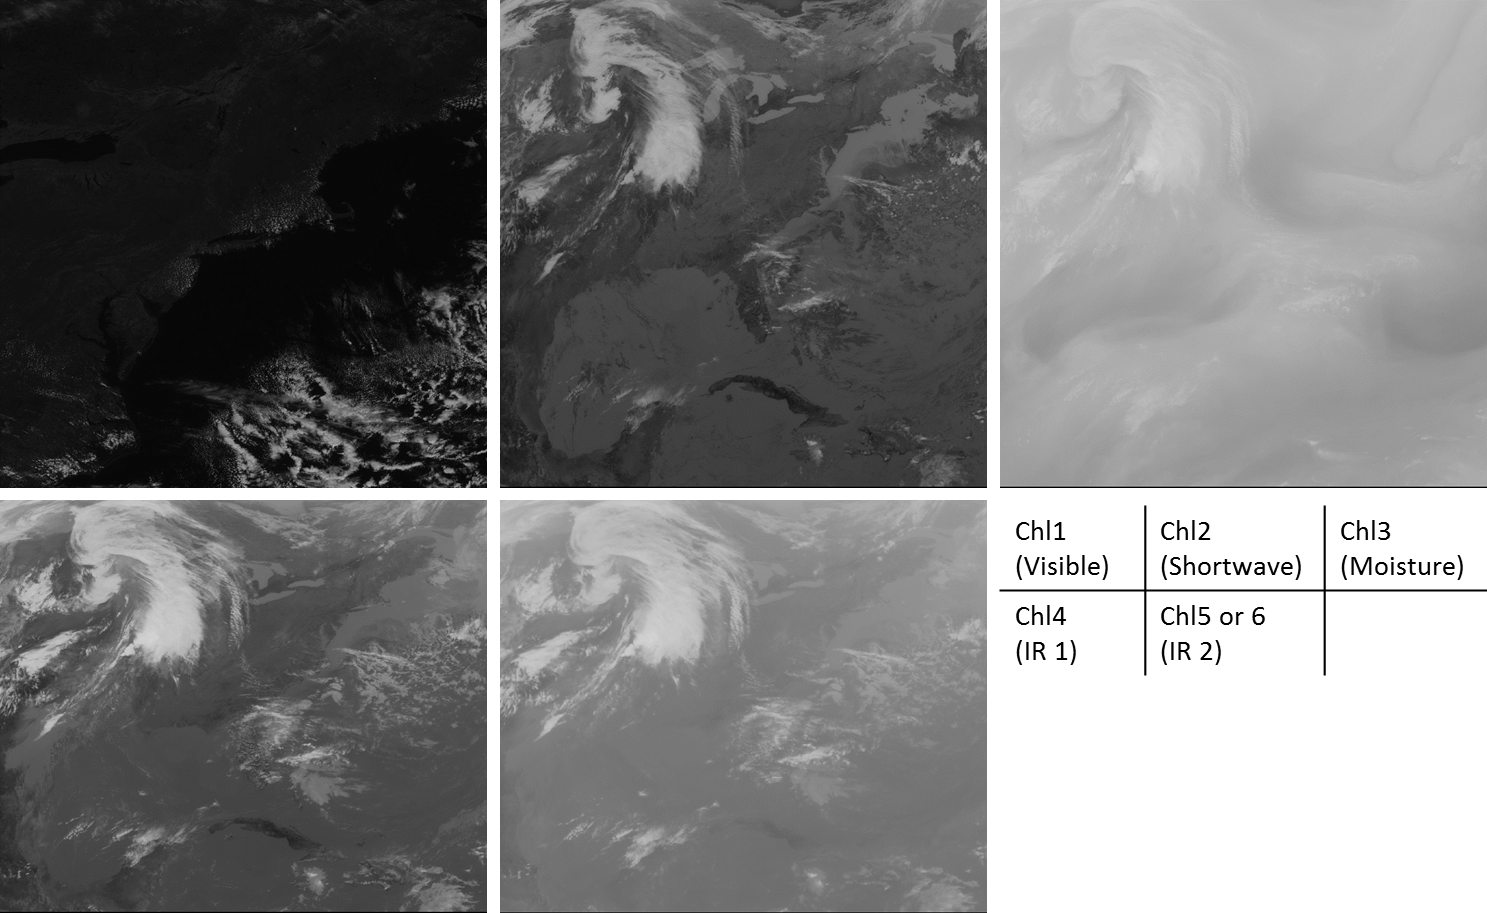
\includegraphics[width=2.5 in]{multi_chl}
\label{fig:multichl}
\end{figure}

With these concerns, our novelties lie in data source, model selecting, and more
importantly, cloud motion forecasting:
 
\begin{enumerate}%[(1)]
\item \textbf{integration of multi-channel}  Besides
visible channel, we import other 4 channels multi-channel data of Geostationary
Operational Environmental Satellite(GOES) imaging system into model. Since each
channel can sense radiant and solar reflected energy in different spectrum
range, comprehensive cloud properties can be presented with multispectral
view.( Figure \ref{fig:multi_chl}).

\item \textbf{Data Preprocessing} Abnormalities and noise are common in both
satellite images and measured radiation especially when multi-channel data is
used. Before feeding to model, filters and other procedures are applied to clean
input data. Besides, regarding radiation from ground station, a non-meteorologic
method is presented to deal with normalization and integration.


% using
% various meorological clear sky models as reference.
% discussed previous works\cite{janjai2005development} we use statistical clear sky model with import
% multi-channel data of Geostationary Operational Environemental Satellite(GOES) imaging
% system into satellite model.

\item \textbf{radiation feature with time} Radiation measured in ground station
can be treated as a miniature of microscale solar energy change. We propose
to add the variation of solar radiation as another concerned feature so as to provide
localized knowledge.

\item \textbf{New model with regression} In previous works related to irradiance
estimation, linear model is widely used with empirical correction for
local variation\cite{perez2002new}. We address it differently using the idea of
SVR which takes both linear and non-linear relation into consideration.

\item \textbf{New motion estimation scheme} As motion tracking is the core
procedure of modeling, our system implements an Optical Flow(OF) motion
estimation algorithm on the basis gradient of grey-scale change. Compared with
traditional algorithms, it is more sensitive to small area change and robust in
shape distortion.
\end{enumerate}

% We provide Support Vector Machine(SVM) learning strategy to do regression on ground-based measurement and preprocessed
% multi-channel data to get estimated solar radiation. Then use optical flow
% motion estimation as cloud forecasting strategy to get view of cloud
% distribution in near future. The combination of forecast cloud distribution and
% time feature of radiation will generate final predicted solar irradiance.



In this paper, previous works and potential approaches are discussed in
Section \ref{sec:bg}. In Section \ref{sec:modeling}, preprocessing scheme and
SVR method is presented in details. Later in Section \ref{sec:forecasting},
motion estimation techniques are discussed and compared. As for details
of satellite model, Section \ref{sec:Models} formulate 7 estimation models
convering linear and non-linear, regular and SVR. In Section \ref{sec:result},
performance of satellite models is presented on aspects of estimation and
forecasting. Based on these results,in Section \ref{sec:conclusion}, we conclude
that the new forecast system has significant improvement in
mid-term radiation forecast field.


% \begin{enumerate}%[(1)]
% \item \textbf{integration of multi-channel}  Instead of
% visible channel only, we import multi-channel data of Geostationary Operational
% Environemental Satellite(GOES) imaging system into satellite model. 
% % Since each channel can sense radiant and solar reflected energy in different
% % spectrum range, cloud properties can be presented more with combination of multi-channel satellite image.
% 
% \item \textbf{New preprocessing approache}  Instead of
% using various clear sky models discussed previous works\cite{Janjai:2005,} we
% use our own non-meteorologic clear sky model with import multi-channel data of
% Geostationary Operational Environemental Satellite(GOES) imaging system into satellite model.
% 
% \item \textbf{radiation feature with time} Radiation measured in ground station
% is a good miniature of microscale solar energy change. We propose to add the
% variation of solar radiation as another concerned feature so as to provide
% robustness with localized knowledge.
% 
% \item \textbf{Max-margin regression} In satellite model field, linear
% model is widely used with empirical correction for local
% variation\cite{Perez:2002}. We address model differently using the idea of
% max-margin regression to improve performance. In experiment, we consider
% both linear and non-linear kernel cases of Support Vector Regression model(SVR).
% 
% \item \textbf{New motion estimation algorithm} Unlike block-based template
% matching, we utilize the optical flow motion estimation as a tool to
% extract cloud motion with concern of gradient of greyscale change within smaller
% range.
% \end{enumerate}

% Out study first introduce current progress of 

\section{Background}
\label{sec:bg}

% On the basis of this correlation, we expand the idea to multi-channel data of
% Geostationary Operational Environemental Satellite(GOES) imaging system.
% Since each channel can sense radiant and solar reflected energy in different
% spectrum range, cloud properties can be extracted with preprocessing and
% combination of multi-channel satellite image. To increase local accuracy, we
As estimating solar radiation data from satellite images is more accurate than
interpolating data measured by a modern radiometric network,\cite{zelenka1999effective}, 
Many works regarding mesoscale range have been develop to do radiation
estimation using satellite data. In early years, Satellite models are built up firstly
to correlate cloud coverage with Global Horizontal
Irradiance(GHI)\cite{cano1986method,stuhlmann1990improvement,schmetz1989towards}.
Later works follows this idea by studying on linear relationship between Direct
Normal Irradiance (DNI) and satellite visible
channel\cite{ineichen1999derivation,hammer2003solar}. These
models use ``Cloud Index"(CI) as optical density derived from satellite data to
indicate fraction or coverage. By using multiple empirical clear sky models,
the local distribution of solar energy is derivable from satellite
image\cite{janjai2005development,martins2007satellite}. More recent
works majorly follow this idea but with different concerns such as terrain
factor\cite{perez2004producing}, but with new ideas coming from knowledge of
other fields such as statistical approach\cite{zarzalejo2009new} and
Artificial Neural Network(ANN) method\cite{zarzalejo2005artificial,csenkal2009estimation},
moreover even without including meteorological data\cite{csenkal2010modeling}.
In fact, the biggest problem of framework of cloud coverage lies in untrusted and unstable visible channel image, since snow coverage and floating brightness of image with various zenith angle. Though Multispectral analysis is the most known and developed
method to detect clouds, this work relies on heuristic thresholds for infrared
and visible range are needed for cloud
classification\cite{ricciardelli2008physical} and snow
detection\cite{perez2010improving} Another drawback of previous works is that simple linear relation derived from cloud coverage has limitations in describing
variation under cloudy condition. Therefore, a customized constant must be
used as an estimation compensation to reduce linear biased influence
\cite{perez2002new}.

On the topic of forecast using satellite, studies are mostly around
cloud prediction. To describe cloud coverage in advance, cloud motion vector
extraction is usually used for estimating cloud movement. As an import input
parameter to feed satellite models. Cloud motion tracking algorithm is
commonly generated from blockwise cross-correlation
matching\cite{leese1970determination,heinemann2006forecasting}. It turns
out to be highly sensitive to block size and segmentation as it try to represent
area of cloud in block unit. In fact, this methodology is based on a basic assumption that cloud motion is stable and identical with no deformation. But in reality,
cloud on satellite image is more complicated as with rotation and shape
changing. Therefore merging and splitting of cloud will be ignored due to fixed
block size. Another extreme case is that when multilayer clouds appear, block
matching will fail as its correlation only covers the texture information in a
block. Therefore a lot of recent works tried evade the unsolved issue of cloud
motion by integration of other source of information,e.g. radar ground measurement.
One way to to predict cloud ahead is using ground radar to get continuous
radiation fluctuation trend\cite{gorsdorf2011cloud}. Another work
explores the time series feature of cloud statistically to do
prediction\cite{yang2012hourly}. The drawbacks of no-motion methodology is that
cloud tracking is of low precision and forecast time can only be either minutes or up to 2 hours as they claimed.
Though satellite approach is also in mesoscale, local information can be
assimilated through adding ground-based pyranometer and multispectral
views.Another drawback of current models is that the precision in
both temporal and spacial aspect decrease rapidly with the longer forecast
period. Due to the restriction of motion estimation algorithm, cloud 

In our approach, we are targeting to use the ground-based pyranometer and
satellite image to get estimated radiation in future. The local instrument
can provide Direct Normal Irradiance(DNI) per second while satellite image
has 30 minutes response time before next scanning. For pre-scheduling
need, radiation forecast coverage starts from 30 minutes to 5 hours. Compared
with pyranometer, satellite image has low spatial resolution(1 km x 1 km in VIS
channel, 4km x 4km in Infrared channel), especially in multispectral
and motion vector related applications. To meet to requirement of local
forecast, pyranometer data is assimilated into satellite model as another
feature. 


\section{Preprocessing and modeling} % 1) need better name 2) re-consider
% better place to put this section
\label{sec:modeling}
In this section, we present the idea of preprocessing pipeline at the beginning.
This procedure is significant for data selecting and noise filtering. In general, preprocessing
includes satellite multi-channel data and radiation data. The need of
radiation data processing originates from ground measurement data normalization
and clear sky calculation.  In later subsection, a new satellite model using SVR
is introduced. Compared with previous linear approaches, we propose a new linear
relation solution using SVR linear kernel. To utilize the SVR more, we also
develop non-linear solution to the forecast problem.


\subsection{Preprocessing}
\label{subsec:preprocessing}
Since remote sensing used in geostationary satellite relies on scanning of
radiometer, in some cases, the capture of will fail due to unresolved reasons.
From the images postprocessed from raw data, it is more obvious and intuitive to
see the errors. Since multi-channel data are proposed to be used as input data,
it is necessary to preprocess images before modeling and prediction further.
From the dataset collected by GOES project[], we find several patterns of error
that appear frequently: 1) black rasters of multispectral images due to failure
of sensing or raw data processing, 2) luminance variation, especially on visible
channel, 3) Multi-channel timestamp mismatch. One solution of preprocessing to
solve these common errors is to use empirical filters such as mean filter and
bad-frame filter. Another one is to regulate the brightness with normalization
with zenith. The overview of preprocessing is shown in Figure
\ref{fig:satprepro}.

Besides preprocessing of satellite data, another key procedure is related to
radiation measured by pyranometer. As ground truth of model output, and maybe
input feature, how to remove noise of radiation is crucial in modeling and
forecasting. With this concern, raw radiation is processed through two modules
in parallel and combined together with using $normalization and integration$
scheme to output fraction of radiation over clear
sky (Figure \ref{fig:satprepro}). Similar to satellite data preprocessing, One
of the modules is responsible for noise removing with filters and thresholds.
Differently, the other radiation module is designed for clear sky irradiance
calculation. 


The importance of clear sky model is that normalization based on clear sky value
indicates the fraction of cloud coverage which is more stable and less
sensitive than radiation value itself which fluctuates with different
atmospheric conditions. But in most clear sky models discussed in \ref{sec:bg},
the calculation of solar direct normal irradiance is based on parameterization
model. In other words, model takes a lot of atmospheric input
parameters such as O2, CO2, ozone, water vapour and aerosol optical thickness
(AOT). The setting up of each model requires peripheral instruments for
additional information. As a result, prediction of radiation change becomes more
challenging in terms of precision and location. Thus we designed a new method
to solve the estimation problem but with less variables involved. With only
historical radiation data, a clear sky model can be estimated using statistical
method,for instance, regression. In our model, 2-order
polynomial regression is used for generation of monthly clear sky curve(figure
\ref{fig:csfig}).


\begin{figure}[tb]
\centering
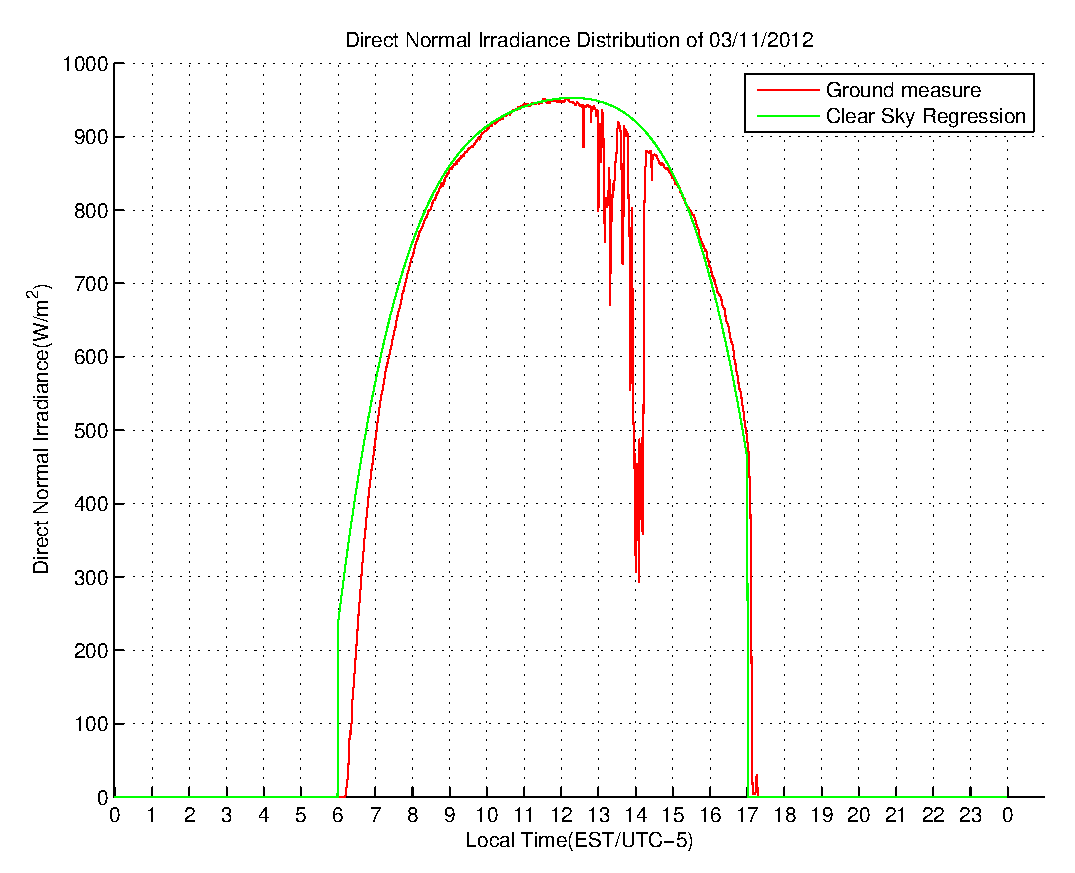
\includegraphics[width=3 in]{csfit}
\label{fig:csfig}
\end{figure}

To combine two models together in final step of radiation preprocessing,
$normalization and integration$ is proposed. $Normalization$ stands for the
calculation of fraction over clear sky value while $integration$
requires radiation and clear sky value at certain point to be
integral over time. The idea of using integral is because of the mismatch of
time range between satellite and ground base station. On one hand, the routine
scan of satellite is 30 minutes while regular pulse of pyranometer is in 1s
unit. On the other hand, As scanning of takes minutes for the whole plate view,
timestamp of satellite is not that accurate. As a result, fluctuation in
between and imprecision of time needs to considered in preprocessing. With
integral around certain period at satellite timestamp, radiation is less
sensitive than picking single value and able to capture the variation during the
span. Then fraction of radiation is calculated using equation \ref{eq:radnorm}.

% Integration between mesoscale data and microscale should cover both temporal and spaticial differences. In satellite dataset, as multi-channel images have different resolution in sensing coverage, coordinate mapping and interpolation are used for unifying pixel scale.
% While in radiation dataset, the sampling rate 1 per second whereas
% satellite update every 30 minutes(routine scan). Therefore, short-term
% fluctuation and noise in 30 minutes cannot be capture by satellite channels due
% to granularity issue of time. Then in the last preprocessing, we implement a
% method using the idea of integral and normalization. The solar radiation at time
% $t$ is the fraction of integral over $2*N$  minutes. The equation is
% \ref{eq:radnorm} while $CSI$ stands for clear sky irradiance calculated from
% clear sky model.

\begin{equation}
DNI_{norm}=\frac{\int_{t-N}^{t+N}DNI}{\int_{t-N}^{t+N} CSI}
\label{eq:radnorm}
\end{equation}

where $2xN$ is the integral period at time $t$.



% GOES data is carefully calibrated after gathering, in multispectral images which are derived from raw data of radiometer, still have several greyscale issues.
% Most servere one is the scanning failure. Satellite imager system may fail to
% capture and leave a black gap on image randomly. This cause big problems in
% motion estimation as most algorithms are texture based. . Another issue is the
% fluctation of brightness on image which makes satellite input more complicated
% and unpredictable. With the need for removing the noise from input, we use
% filters to remove the gap of image or get rid of noisy image at certain level.
% Another key procedure of preprocessing is the radiation value from ground
% measurement. The basic idea of radiation processing is to remove noise and
% build up clear sky radiation estimation as a reference of no-cloud situation.
% The calculation of solar direct normal irradiance is based on parameterisation
% model. This model takes a lot of atmospheric input parameters such as O2, CO2, ozone, water
% vapour and aerosol optical thickness (AOT). It means that other instruments
% and esitmation model will be needed for forecast part. With more uncertainties
% of atmosphere conditions imported into forecasy system, it is more chanllenging
% to predict radiation change. Therefore we develop a new clear sky calculation
% model in preprocessing part with regression statistically. One advantage of this
% methodology is that local measurements of atmosphere are not necessary. The
% computation is only based on historical radiation data. Overview of algorithm
% structure is listed in \ref{fig:satpre}.



% Clear sky 
% 
% ThSince the aim of radiation
% forecast is based on radiation and satellite only clear sky case previous approaches focus on using empirical In our system, different from previous approach using clear sky model with meteorologic parameters as inputs\cite{perez2002new}, we consider  preprocessing work is to find clear sky Upon the analysis of channel variation with solar angle change, we use normalization to decrease the influence of total brightness
% 
% In our system, 

% preprocessing such as data
% selection and normalization are needed before any further analysis. Before the feeding into model, previous radiation is imported To better understand relation between satellite multi-channel data and solar irradiance, our approach is different with several
% and either or using radar as another source of ground measurement[Gorsdorf, U.
% 2011] using N Under the limitation of instruments and 
\subsection{SVR modeling}
\label{subsec:SVR}

With preprocessed input data of both multispectral images and radiation feature,
we summarise modeling as a regression problem with a set of training
patterns $(x_{1},y_{1}),\ldots,(x_{n},y_{n})$, where $X_{i} \in R^{N}$,
i=1,\ldots,n.
Specifically in our concern of satellite model, the idea is implemented as:
$y_{t} \leftarrow x_{t}, x_{t}=\{Chl1_{t},Chl2_{t}, Chl3_{t}, Chl4_{t}, Chl6_{t}, y_{t-\Delta t}\}$
,where $Chln$ stands for satellite channel n, $y$ is DNI value from
preprocessing. If the relation is linearly formulated, the estimation output is
presented in (\ref{eq:lifx}) as a function of $(w,b)$. $\left \langle . \right
\rangle$ stands for dot product.

\begin{equation}
f_{t}(x)=\left \langle w,x_{t} \right \rangle + b ,w \in R^{N},b\in R
\label{eq:lifx}
\end{equation}

To solve this problem, we use Support Vector Regression(SVR). SVR utilize the
idea of maximum margin with regularization of cost function. The solution of SVR
can be treated as a classic quadratic optimization problem. In general, it is
equivalent to solve:


% To solve the problem and import non-linear relation into estimation, we turn to use Support Vector
% Regression(SVR) on the basis of Support Vector Machine(SVM). In machine
% learning field, SVM has been widely used for classfication and labeling.
% The basic idea of SVM is formed in 1992\cite{boser1992training}. In 1995,
% Corinna Cortes and Vladimir N. Vapnik expand the idea to modified maximum margin
% with cost function penalty on mislabeled examples\cite{cortes1995support}. As
% a extension of SVM for regression, SVR is firstly developed for various forecast
% problems in 1997\cite{drucker1997support}.
% 
% Among different types of SVR methodologies, the most commonly used is
% $\epsilon$-SVR which consider a $\epsilon$-sensitivity tube by a regularization
% technique that considers $\epsilon$ deviation from $y_{t}$ at the same time
% flatness of regression\cite{vapnik1999nature}. In detail, points that lie
% outside certain bound that defined by $\epsilon$-sensitivity tube from
% regression are penalized in ojective funtion. With slack variables imported, the
% satellite model regression will be formalted as an optimization problem:


\begin{equation}
\begin{split}
\label{eq:liopti}
minimize\quad \frac{1}{2}\left \| w \right \|^{2}+C\sum_{i=1}^{n}(\xi_{i} +
\xi_i^* ) 
\\ subject \, to \quad 
\begin{Bmatrix} 
y_i-\left \langle w,x_i \right
\rangle -b\leq \epsilon+\xi _i \\ \left \langle w,x_i \right \rangle - y_i+b\leq \epsilon+\xi _i^*
\\ \xi _i,\xi _i^*\geq 0
\end{Bmatrix}
\end{split}
\end{equation}


SVR is also useful for non-linear problem as it uses non-linear kernels. The
kernel of SVR is a mapping method which can be transferred as linear relation.
Once the linear relation is defined from kernel mapping, quadratic optimization
problem can be solved without additional modification on objective function and
constraints. In this paper, we use a kernel named radial basis
function(RBF) for our non-linear modeling. The $f(x)$ in RBF concern is
rewrite in (\ref{eq:RBFfx}) .With RBF kernel, the estimation formula
is different from previous linear SVR approach, since it contains a mapping of $x_{i} \leftarrow
\Phi(x_{i})$. In RBF method, $\Phi(x_{i})$ is implicit mapping and can be
ignored through kernel $k(.,.)$,defined in (\ref{rbfkernel}) calculation in
optimization.

\begin{equation}
% f_{t}(x)=\left \langle w,\phi(x_{t}) \right \rangle + b ,w \in R^{N},b\in R
f_{t}(x)=\left \langle w,\phi(x_{t}) \right \rangle + b 
\label{eq:RBFfx}
\end{equation}


\begin{equation}
\label{rbfkernel}
k(x,x^{\prime})=\left \langle \phi(x),\phi(x^{\prime}) \right \rangle
=e^{-\frac{\parallel x-x^{\prime} \parallel^2}{2\delta^2}}
\end{equation}

In SVR model calculation, an Open source library named LIBSVM\cite{CC01a} is
used to solve the optimization problem given satellite data and radiation
values. The optimal solution is then generated through tuning regularization
parameters.



% \begin{equation}
% \begin{split}
% maximize\quad 
% \begin{Bmatrix} -\frac{1}{2}(\alpha_{i}-\alpha_{i}^{*})(\alpha_{j}-\alpha_{j}^{*})k(x_i,x_j) 
% \\ -\epsilon\sum_{i=1}^N(\alpha_{i}-\alpha_{i}^{*})+
% \sum_{i=1}^{N}yi(\alpha_{i}-\alpha_{i}^{*})
% \end{Bmatrix}
% \\ subject \, to \quad \sum_{i=1}^N(\alpha_{i}-\alpha_{i}^{*})=0\,and\,
% \alpha_{i},\alpha_{i}^* \in[0,C]
% \end{split}
% \end{equation}
% the solution is:
% 
% \begin{equation}
% w=\sum_{i=1}^{N}(\alpha_{i}-\alpha_{i}^{*})\phi(x_i)\;and\;f(x)=\sum_{i=1}^{N}(\alpha_{i}-\alpha_{i}^{*})k(x_i,x)+b
% \end{equation}

% lthough cloud information is predictable in
% numerical weather prediction Besides, since satellite images are all mesoscale
% view generated from radiometer in high altitude, it leads to a big challenge of
% accuracy when comes to local solar plant scheduling and planning. Therefore We
% propose to combine ground station radiation as local view with satellite
% multi-channel data. With these concerns, we develop a new model with visible
% chanel and 4 infered channels using Support Vector Machine as the regression
% tool to consider both linear relation and non-linear relation. SVM is widely
% used in data mining  field as a classfication method based on mmaximum-margin
% hyperplanes\cite{boser1992training}. A version of SVM for regression is firstly
% presented in 1996[Drucker 1996]. With these considerations, we develop a new
% model with visible chanel and 4 infered channels using Support Vector Machine as
% the regression tool to consider both linear relation and non-linear relation.
% SVM is widely used in data mining field as a classfication method based on
% maximum-margin hyperplanes[boser 1992]. 


\begin{figure}[tb]
\centering
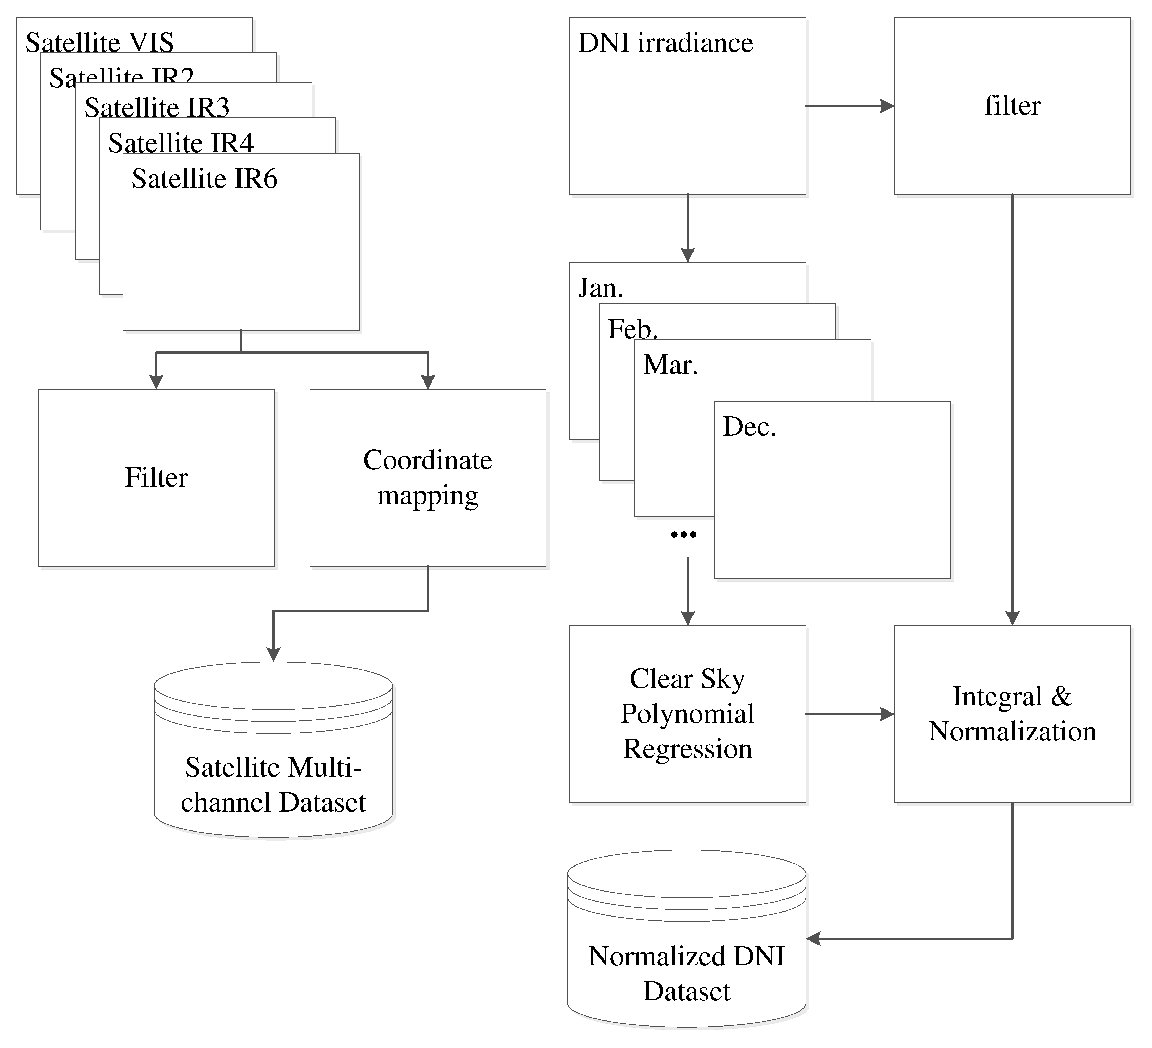
\includegraphics[width=3 in]{satprepro}
\label{fig:satpre}
\caption{Data Preprocessing Framework}
\end{figure}

\section{Motion Estimation and forecasting}
\label{sec:forecasting}
Forecasting part in this paper is equivalent to capturing radiation feature with
time and cloud tracking. The radiation related prediction uses previous
radiation directly as pre-knowledge of prediction while cloud tracking relies
on motion estimation on satellite image. The goal of using satellite image is to
get the movement of cloud field and predict cloud location after minutes
or even hours. Thus, algorithms of motion estimation are crucial for precision
of forecasting output. In this section, we propose to use Optical Flow(OF)
motion estimation method as the core of tracking algorithm. To better illustrate
the performance of it, a comparison is done with another common method using
block-matching.

% In this section, tracking methods of cloud is discussed in detail.  As
% our approach of prediction rely on images only, an Optical Flow(OF) motion estimation
% methodology is introduced. Compared with block matching algorithm, Optical
% Flow is more stable in motion tracking and able to capture changes in pixel
% scale.

\subsection{Optical Flow Motion Estimation}
\label{subsec:OF}
% Motion estimation techniques are widely used for video coding and compressing in
% image processing field. The common goal has been set to reduce temporal
% redundancies so as to get predicted image with lower cost in both storage and
% computational time. Thus feature based methods such as block-matching are
% widely used to meet criteria of minimum cost. Whereas, in satellite forecast
% application, the focus is more on accurary of motion vector extraction. 
As motion estimation is not a new topic since in image processing and multimedia
field, a lot of approaches have been carried out. The most common method is
blockwise motion estimation which is based on block similarity to estimation
displacement of each block. This approach is widely used in video coding and
compressing as its properties of fast speed and high compressing ratio. But the
performance of block related algorithms is very sensitive to region and feature
matching which assume consistence of segmentation and luminance in region. In
other words, with cloud variation and uncertainty on satellite image, block
matching is very unstable varying with blocksize and similarity criteria. As a
result, to get rid of these issues in satellite application, we turn to use
Optical Flow algorithm after comparing with traditional block matching.

Optical Flow Motion Estimation is a branch of methodology that utilize the
gradient of image. Under the assumption of constant illuminance, displacement of
image will be estimated through ingredient change. Optical Flow has a lot of
variations as ingredient of image is defined differently. In our approach, we
choose Lucas-Kanade Optical Flow(LKOF)\cite{lucas1981iterative} as the tracking method. To
improve the robustness of motion tracking on satellite image, we implement a pipeline which
use recursion to approach the best tracking result. Visible channel image is
scaled into several layers size(in experiment 1000x1000, 500x500 are used), for
smaller image(Upper layers in image pyramid) with higher ratio, OF tracking is
applied for detecting motion vectors. This motion vector will be initial motion
vector to the next layer. The final layer is normally with no scaling, OF is
recursively done with the direction of gradient change. Then final motion vector
map is generated for each pixel. In reality, window size and number of layers
need be to tuned in case of over-estimation. The overview of pipeline is
presented in Figure \ref{fig:OFME}.


% In feature or region based motion tracking, algorithms use different criteria as
% similarity measurement between regions or blocks. In general all the methods
% rely on an assumption of consistence of region and luminance. Although
% normalized cross correlation has been applied to avoid luminance bias, they
% performance are not stable as proper segmentation of regions are required.
% On satellite images, Relying on cloud detection may have contrary influence on
% cloud motion tracking since detection and classification introduce other
% uncertainties, eg. differtiation of snow and cloud. 
% 
% Optical Flow estimation is a branch of methodology that utilize the gradient of
% image. The core of algorithm is the assumption of constant illuminance.
% Displacement of images will be presented and estimated through ingredient
% change. Just like different criteria in region based motion tracking,
% various Optical Flow methods implements ingradient in unique way. In this paper,
% the most common method named Lucas-Kanade Optical Flow(LKOF) is implemented.
% In order to improve accurary of motion vector extraction, the tracking is
% recursive following the ingredient change. As suggested in image processing
% filed, motion estimation process also implement the tuning of pyramid of
% image(multi layer images) and ingredient windows size.

\begin{figure}[tb]
\centering
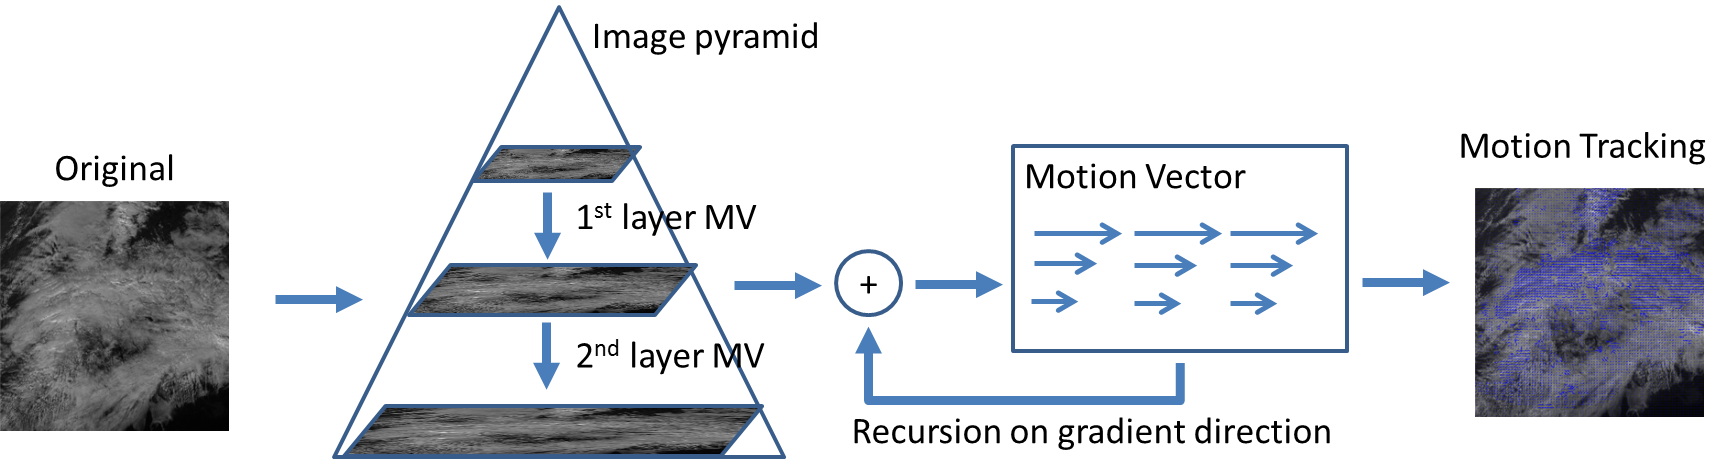
\includegraphics[width=3 in]{OFME}
\caption{Optical Flow Motion Estimation Pipeline}
\label{fig:OFME}
\end{figure}




%Different from texture based matching us

%Optical Flow Motion Estimation algoritm is developed based on an assumption of is a scheme used


%In order to The major challenge to feature based algorithms is the segmentation and cloud extraction

\subsection{Optical Flow vs. Block-based matching}
\label{subsec:DFDresult}
To illustrate the difference, we design two experiments to compare Optical Flow
with Block Matching method in both image scale and pixel scale. To measure the
goodness of motion estimation, the most straightforward method is to use
output motion vectors directly to generate predicted image and compare with
ground truth image. Based on this idea, Displaced Frame Difference(DFD) is used
as benchmark of compare two images. In this paper, $DFD_{avg}$ is generated
by averaging $DFD$ over all pixels(\ref{DFD}). 
% In image processing field, Displaced Frame Difference(DFD) is widely used as benchmark for motion estimation evaluation. DFD is calculated by sumation over difference on
% predicted image(original image with displacement). In pratical usage, DFD
% value is calculated with average over all pixels to make sure DFD streching
% from 0 to 255. With $u$,$v$ standing for motion vector in $x$,$y$ direction and
% $N$ as total number of pixels, the equation of average DFD is described in
% \ref{eq:DFD}. 

\begin{equation}
DFD_{avg}=\frac{\sum_{i,j}\left |I_t(i,j)-I_{t-\Delta t}(i+u_{i,j}\Delta
t,j+v_{i,j}\Delta t)\right |}{N}
\label{eq:DFD}
\end{equation}

where $u$,$v$ is motion vector of pixel $(i,j)$ in direction of $x$,$y$,
respectively.

Block Matching method used for comparison is Hierarchical Block-Matching(HBM).
It uses bigger block(50 x 50 pixels) as the representative of smaller block(10
x 10 pixels) to decrease influence of noise in small area. The similarity is
defined as normalized cross correlation. As a result, HBM generates motion
vectors in unit of 10 x 10 resolution. In LKOF method, we take 10 X 10 region
as gradient calculation, 2 layer pyramid, and up to 100 iterations to generate
pixel-scale motion vectors. The comparison of DFD score is shown in Figure
\ref{fig:DFD}. The result shows that Optical Flow with mean filter is better in
motion tracking.

DFD score, however, is a criteria per image which consider the whole image as
unit. It means that DFD is not able to present the goodness of slow motion or
motion in small scale. In addition, as a sum of absolution error, it puts
more weight on no motion detection because motion since movement of pixels
leaves gap( black area) in previous position. But this should not be encouraged
especially motion is not that obvious. Therefore, we pick another criteria to
get evaluation of prediction results in local view. In \ref{sec:result}, we use
satellite model to output forecast radiation based on predicted images, with
ground truth from local station, a evaluation can be presented with
deviation in terms of radiation.


% region matching as small blocks(10 x 10 pixels) are represented by (50 x 50
% pixels) using normalized cross correlation as similarity. On the other side,
% LKOF algorithm is a pixel-scale estimation technique therefore the prediction
% using motion vector will leave lots of black holes as information lost. We use
% mean filter to fill the holes to make image continous and smooth. The test
% result of DFD is shown in Figure. \ref{fig:DFD}. What should be noted about DFD
% is that to some extent, it has the ability to show motion estimation precision
% in general. But One common drawback of DFD benchmark is that it is passive
% in prediction. In other words, no motion will be encouraged in short term to
% preserve good performance in average errors. From the test of DFD, the optical
% flow with mean filter is better in motion tracking in mesoscale application.
% This is also proved when using SVR model as another benchmark in
% \ref{sec:result}. As a make-up to DFD criteria, SVR model is local
% scale measurement of goodness of motion estimation algorithms verified by
% ground-truth radiation.



\begin{figure}[h]
\centering
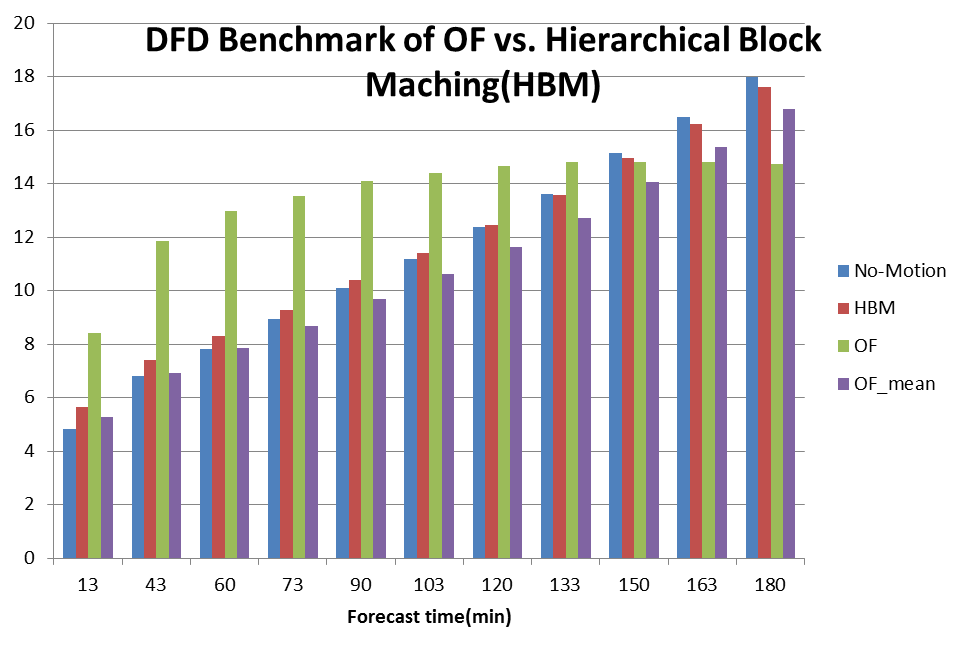
\includegraphics[width=3 in]{DFD}
\label{fig:DFD}
\caption{DFD score of OF vs. HBM}
\end{figure}

\section{Radiation Prediction Models}
\label{sec:Models}

As mentioned in \ref{subsec:SVR}, satellite model is formulated as
$y_{t} \leftarrow x_{t}, x_{t}=\{Chl1_{t},Chl2_{t}, Chl3_{t}, Chl4_{t},
Chl6_{t}, y_{t-\Delta t}\}$. The $y_t = f(x_t)$ mapping can be linear or
non-linear. In single-channel model, linear relation is commonly used for cloud
coverage extraction. While in multi-channel approaches, non-linear idea is
also accepted since input data dimension increases more than 5. In this paper, 7
of satellite models are implemented for estimation and forecasting evaluation.
On the whole, 5 of them still stick With linear exploration while 2 of them try
to consider the problem as non-linear. In the view of input data, 2 linear
models are built directly on visible channel , others utilize
multi-dimension input data.

For comparative study, we use Cloud Index(CI) model as our baseline. This is a
widely used estimation model on the bais of linear relation between
single-channel with radiation. One drawback of this model is the normalization
since dynamic range of channel with time is not stable and visible channel may
have brightness variation. Driven by this idea, two extensions are implemented
with modifications: 1) normalization with zenith, 2) removal of
compensation for bias error. The first extension is Linear Regression(LR). It
considers visible channel with regression method instead of calculate CI first.
The other one is Aggregate Linear Regression(ALR) which is linear regression but
with multi-channel data. CI,LR,ALR, are all non-SVR approaches since no
SVR optimization is involved.

The rest 4 models are all SVR models. Similar to as ALR, SVR models also take
multispectral data into consideration. In first two approaches, SVR uses linear
kernel($SVR-Li$) and RBF kernel($SVR-RBF$) to estimation radiation with only
satellate data as input. Driven by the idea of radiation with time feature, two
other SVR models are developed using satellite data and previous radiation as
input. One is extended from linear kernel named as ($SVR-Li_{rad}$) and the
other is from RBF kernel($SVR-RBF_{rad}$). Moreover, another concern in modeling
is that with multiple dimension of input and uncertain quality of motion prediction, output of radiation can be noisy and
outbound. In other words, with normalized radiation as training data, model can
output abnormal values like below lower bound 0 or beyond upper bound 1. Thus,
for the sake of range control, final output of $SVR-Li_{rad}$ and
$SVR-RBF_{rad}$ is trimmed with threshold.

 
\begin{enumerate}%[(1)]
\item \textbf{Cloud Index(CI)} Implementation of CI model is
following \cite{perez2002new} but with our statistical clear sky model.

\begin{equation}
CI=\frac{x_{1}-bound_{min} }{bound_{max}-bound_{min}},x_{1}\in[0,255],
\end{equation}
\begin{equation}
f(x)=w(1-CI)+b,CI \in
[0,1]
\end{equation}

% where $b$ is called the compensation value.

\item \textbf{Linear Regression(LR) on single channel}   LR implements directly
on visible channel.

\begin{equation}
f(x)=wx_{1}+b,x_{1}\in[0,255]
\end{equation}
 
\item \textbf{Aggregate Linear Regression(ALR) on multi-channel} 5 GOES channel
are used for linear regression for radiation. 

\begin{equation}
f(x)=\left \langle w,x \right \rangle+b,x\in[0,255]^{5}
\end{equation}
 

\item \textbf{SVR using Linear kernel($SVR-Li$)} This model
use $\epsilon$-SVR method with linear kernel.

\begin{equation}
% Objective function:\quad f_{t}(x)=\left \langle w,x_{t} \right \rangle + b ,w
% \in R^{5}
f(x)=\left \langle w,x \right \rangle + b, w \in R^{5},x \in [0,255]^{5}
\end{equation}


\item \textbf{SVR using Radial Basis Function kernel($SVR-RBF$)} The RBF funtion
is used for kernel mapping in SVR before linear optimization.

\begin{equation}
f(x)=\left \langle w,\phi(x) \right \rangle + b ,w \in R^{5},x \in [0,255]^{5}
\end{equation}

\item \textbf{SVR using Linear kernel with radiation ($SVR-Li_{rad}$)}
Different from SVR-Li, this model uses previous radiation as another input feature.
A 0~1 threshold of is applied to forecast output to generate normalized
prediction.

\begin{equation}
\begin{split}
f_{t}(x)=\left \langle w,x_{t} \right \rangle + b ,w
\in R^{5},\\
x_t=\{x_{t1},x_{t2},x_{t3},x_{t4},x_{t6},y_{t-\Delta t} \}
\end{split}
\end{equation}
where $x_{tn}$ is input of channel $n$ at time $t$,$y$ is ground truth
radiation, $\Delta t$ is the time span. 
\item \textbf{SVR-Radial Basis Function kernel with radiation ($SVR-RBF_{rad}$)}
Same as $SVR-Li_{rad}$ but with RBF kernel as non-linear mapping to linear
space.

\begin{equation}
\begin{split}
f_{t}(x)=\left \langle w,\phi(x_{t}) \right \rangle + b ,w
\in R^{5},\\
x_t=\{x_{t1},x_{t2},x_{t3},x_{t4},x_{t6},y_{t-\Delta t} \}
\end{split}
\end{equation}

\end{enumerate}


 
\section{Experiment Results} % 1) need better name 2) re-consider better place to put this section
\label{sec:result}

\subsection{Dataset}
\label{subsec:dataset}
The time range of our satellite dataset is from April 1st 2012 to November 1st
2012, covering partial Spring ,Summer, and most autumn. All the raw satellite
multi-channel data is collected from public FTP server from GOES project[].
The radiation data is from pyranometer on-site measurement. As satellite data from GOES has
routine scan(30 min) and rapid scan(15 min), Span between two images is not
fixed and motion vector extraction also takes this into account for later
forecasting. For both satellite images and pyranometer measurement, raw input
has been preprocessed by removing data points which have 1) bad-frame of multi-channels
2) failure of ground radiation sensor 3) multi-channel timestamp mismatch 4) low
solar angles. In total, training dataset is of 8477 frames for each satellite
channel. The timestamps of data records are continous in each individual day
but may not cover all days for each month in range. All radiation data are
normalized and integrated over 15 minutes around frame time of satellite data.
The detailed information of dataset is listed in Table \ref{tab:dataset}.

\begin{table}[htb]
\caption{Satellite Model Dataset}
\centering
\label{tab:dataset}
    \begin{tabular}{   l  |  l  |  l  | l }
    \hline
   Dimension	&size	&temporal resolution	&spatial resolution  \\ \hline
   Channel 1	&8477   &15min,30min			&1km x 1km    \\ \hline
   Channel 2,3,4,6	&8477   &15min,30min		&4km x 4km    \\ \hline
   radiation	&8477   &15min			&NA    \\ \hline 
   \hline
    \end{tabular}
\end{table}


\subsection{Estimation Evaluation}
\label{subsec:esti_e}

For whole satellite model dataset, we used 5-fold cross validation for 7 models
listed in section \ref{sec:Models}. With the purpose of performance evaluation
of models, motion tracking and cloud prediction are skipped in case of
bringing forecast errors. In order to measure the deviation of model output from
ground truth radiation value, Mean Square Error(MSE) and Mean Absolute
Error(MAE) are used to evaluate accurary. They are defined
as:

\begin{equation}
\label{eq:MAE}
MAE=\frac{i}{N} \sum_{i}^{N}\left | f(x_i) - y_i \right |
\end{equation}

\begin{equation}
\label{eq:MSE}
MSE=\frac{i}{N} \sum_{i}^{N}{(f(x_i) - y_i)^{2}}
\end{equation}

Where $f(x_i)$ stands for model estimation radiation using $i_{th}$ data record,
$yi$ is the actual value in accordance with $i_{th}$timestamp, $N$ is the size
of dataset, specifically, $N = 8477$ in experiment. 
Moreover, as radiation is normalized as a fraction of clear sky value, the
fluctuation range is fixed in 0~1. MAE and MSE value only indicate the
percentage deviation of estimation from reality. The final results are shown in
figure \ref{fig:modelsmse} and figure \ref{fig:modelsmae}.


\begin{figure}[h]
\label{fig:modelsmse}
\centering
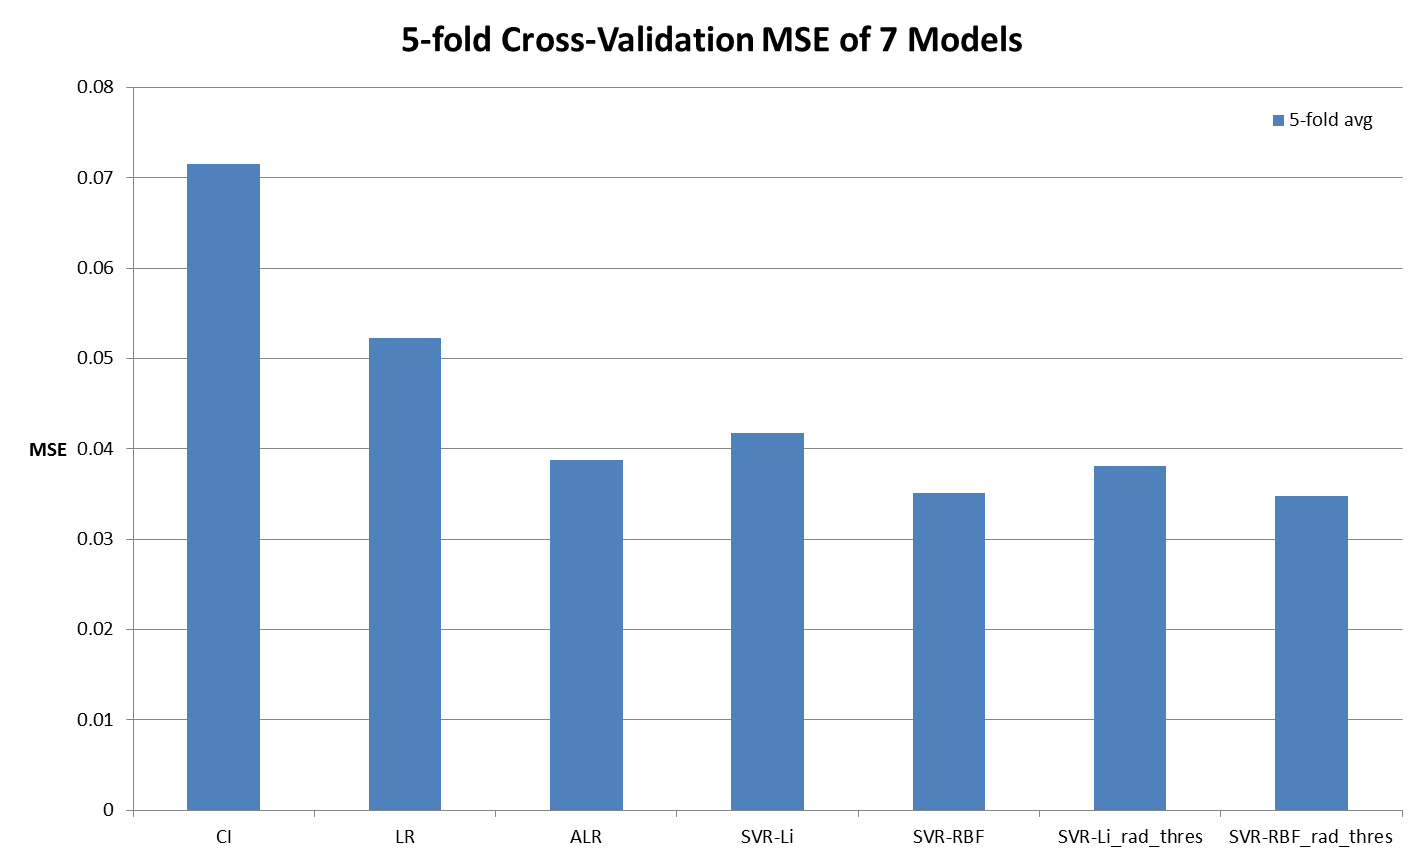
\includegraphics[width=3 in]{modelsmse}
\caption{Averge MSE Plot of 5-fold cross validation}
\end{figure}


\begin{figure}[h]
\centering
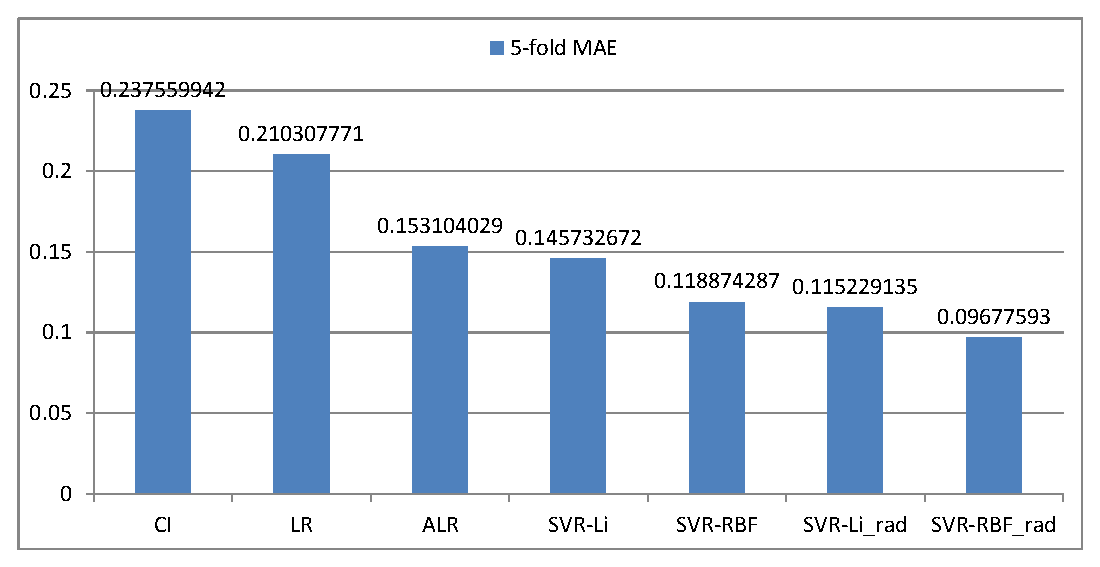
\includegraphics[width=3 in]{modelsmae}
\label{fig:modelsmae}
\caption{Averge MAE Plot of 5-fold cross validation}
\end{figure}
 

\subsection{Forecast Result}
\label{subsec:forecast_e}
As the key procedure that influence accuray of forecasting, motion tracking and
image prediction are taken into evalutaion. Motion vectors extracted from motion
estimation methodology is used for image prediction. With targeting the hours's
forecast to meet mid-term requirement, the experiment is designed
to compare prediction output at 30 mintues,1 hour, 2 hour ,3 hour, 4
hour and 5 hour. 

Besides the purpose of comparison among models, forecasting output is also used
for evaluation of motion estimation algorithms. As DFD value is a measurement of
average error per image, MSE score of local scale(individual pixel) using SVR
model is generated for performance comparison of motion estimation with time.
The result is presented in Figure \ref{fig:mepred}. By using Optical Flow
as motion estimation algorithm, the MSE and MAE score of 7 models is shown in
Figure \ref{fig:modelsmse_pre} and Figure \ref{fig:modelsmae_pre}.

\begin{figure}[h]
\centering
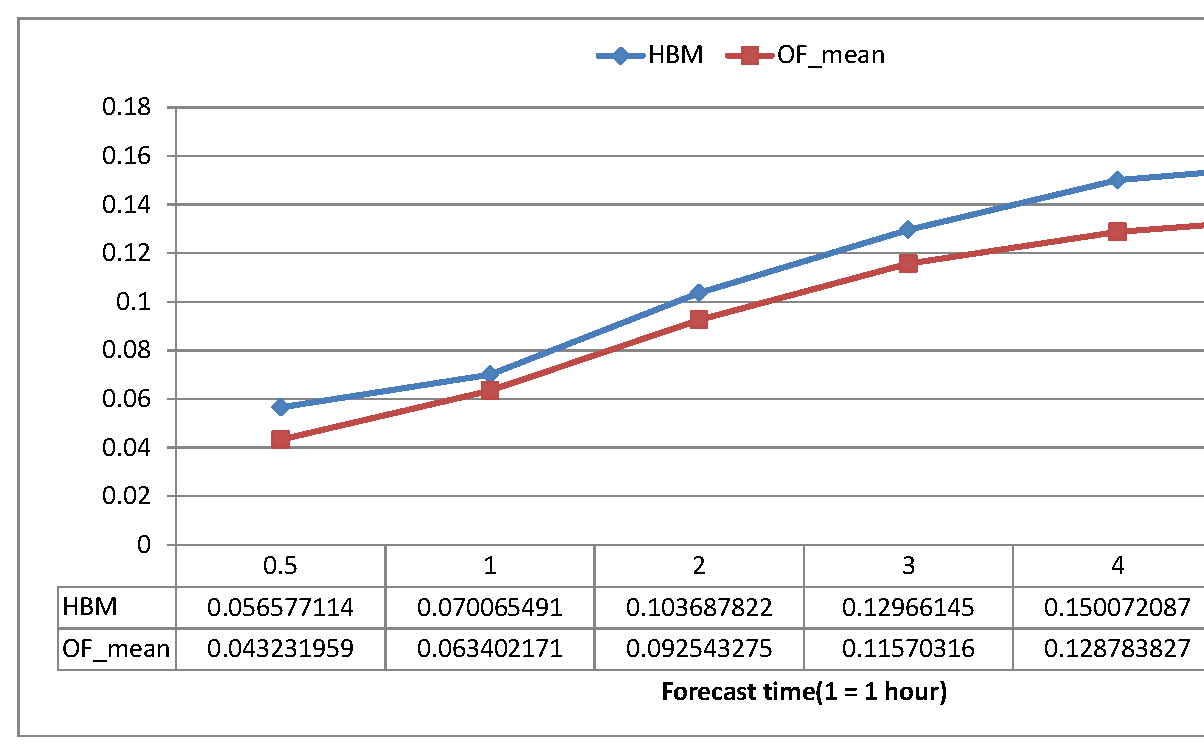
\includegraphics[width=2.5 in]{mepred}
\label{fig:mepred}
\caption{MSE score of Motion Estimation with $SVR-RBF_{rad} Forecasting$}
\end{figure}

\begin{figure}[h]
\centering
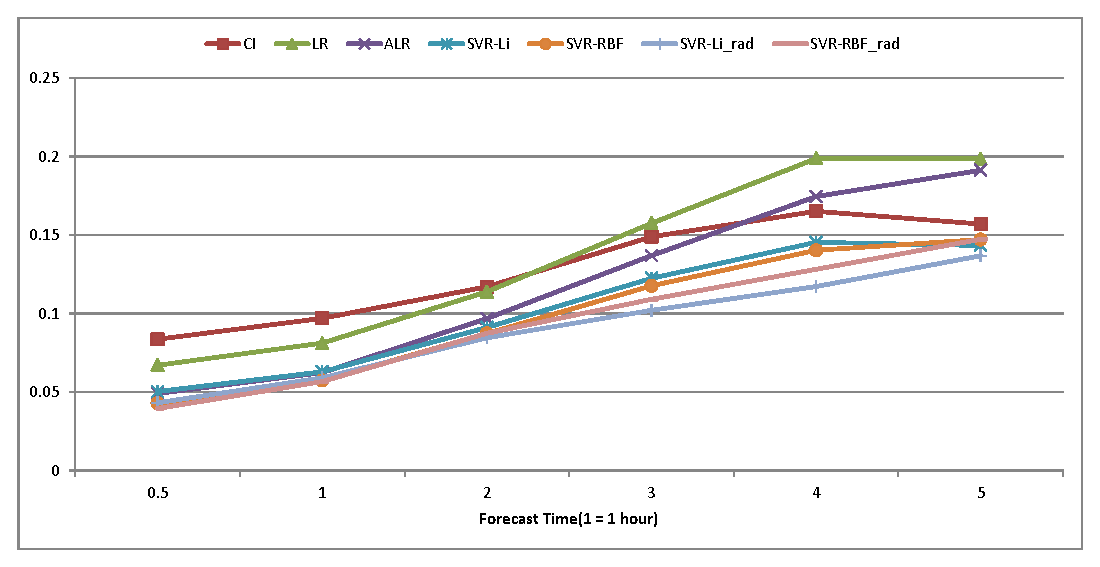
\includegraphics[width=3 in]{modelsmse_pre}
\label{fig:modelsmse_pre}
\caption{MSE score of 7 forecasting models}
\end{figure}

\begin{figure}[h]
\centering
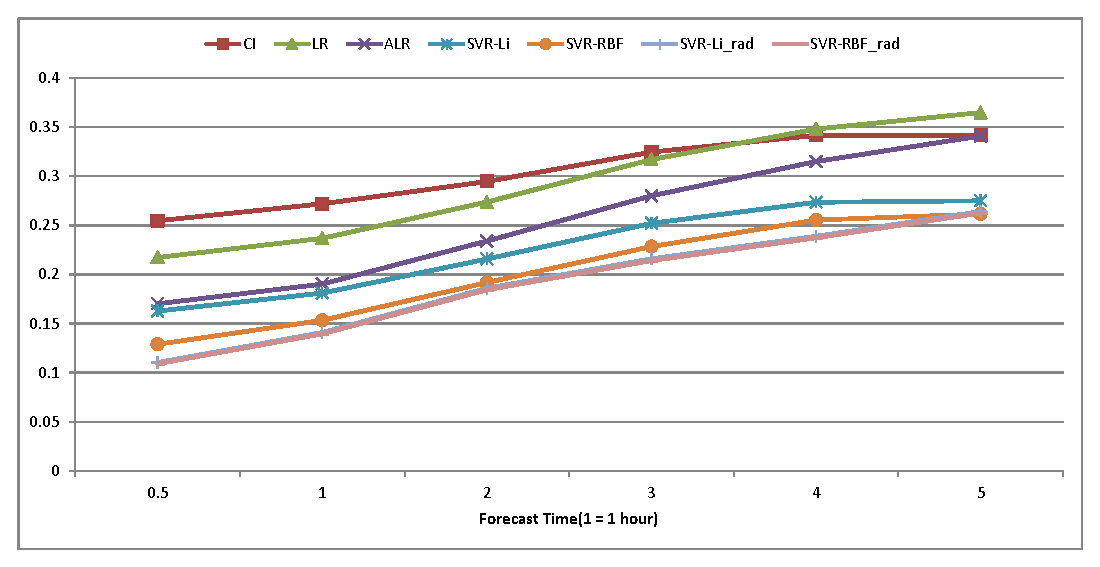
\includegraphics[width=3 in]{modelsmae_pre}
\label{fig:modelsmae_pre}
\caption{MAE score of 7 forecasting models}
\end{figure}


\section{Conclusion} % 1) need better name 2) re-consider better place
% to put this section
\label{sec:conclusion}


In this paper, a new mid-term forecast system is developed with innovations on
both modeling and predicting aspect. To choose and compare satellite
models, we implement 7 methods with both linear and non-linear concerns. From
experiment, we conclude that non-linear SVR model combined with radiation feature is the
best model which has more than $50\%$ than the baseline CI method. In
cloud motion estimation, Optical Flow with mean filter method is used as it is
better than traditional block matching method using both image processing
criteria and forecasting MSE score. In 0.5 ~ 5 hours forecasting, we find
that SVR related models significantly improve the accuracy than others. Although
noise from cloud prediction increase exponentially with time, the SVR non-linear
model is more robust than the baseline,especially combined with radiation at
previous timestamp. The accuracy improvement of is more than $50\%$ in 30
minutes prediction and  $10\%$ in 5 hours prediction.




\bibliography{document}
\bibliographystyle{IEEEtran}
%\bibliographystyle{plain}
%\bibliography{IEEEabrv,IEEEexample}



%\begin{thebibliography}{99}
%\begin{thebibliography}{1}
% \bibitem {Janjai09}
% Janjai S, Pankaew P, Laksanaboonsong J. \emph{A model for calculating hourly global
% solar radiation from satellite data in the tropics}, \hskip 1em plus 0.5em minus 0.4em\relax  Applied Energy 86.9 (2009): 1450-1457.
% 
% \bibitem {Janjai09}
% Janjai S, Pankaew P, Laksanaboonsong J. \emph{A model for calculating hourly global
% solar radiation from satellite data in the tropics}, \hskip 1em plus 0.5em minus 0.4em\relax  Applied Energy 86.9 (2009): 1450-1457.

%WB Rossow, LC Garder - Journal of Climate, 1993 – journals.ametsoc.org
%P Minnis, PW Heck, DF Young - Journal of the atmospheric …, 1993 -
% journals.ametsoc.org E Zaunick, J Levenhagen, K Janschek - 2011 – lib.physcon.ru
%RL Bankert, C Mitrescu, SD Miller… - Journal of applied …, 2009 –
% journals.ametsoc.org 
%[5]Janjai, S., P. Pankaew, and J. Laksanaboonsong. "A model for calculating
%hourly global solar radiation from satellite data in the tropics." Applied
% Energy 86.9 (2009): 1450-1457.
% [6] S¸ enkal O, Kuleli T. Estimation of solar radiation over Turkey using artificial
% neural network and satellite data. Applied Energy 2009;86(7e8):1222e8.
% [7]Zarzalejo LF, Ramírez L, Polo J. Artificial intelligence techniques applied to
% hourly global irradiance estimation from satellite-derived cloud index. Energy
% 2005;30:1685e97.
% [8] S¸ enkal O. Modeling of solar radiation using remote sensing and artificial neural network in Turkey. Energy 2010;35:4795e801.
% Cano, D. et al., 1986. A method for the determination of the global solar radiation from meteorological satellite data. Sol. Energy 37 (1), 31–39.
% Perez, R. et al., 2002. A new operational satellite-to-irradiance model—description and validation. Solar Energy 73 (5), 307–317.
% Schmetz, J. (1989): Towards a Surface Radiation Climatology: Retrieval of Downward Irradiances from Satellites. Atmos Res., 23, pp. 287-321
% Stuhlmann, R., Rieland, M., Raschke, E., 1989. An improvement of the IGMK model to derive total and diffuse solar radiation at the surface from satellite data. J. Appl. Meterol. 29, 586–603.
% Ineichen, P., Perez, R., 1999. Derivation of cloud index from geostationary satellites and application to the production of solar irradiance and daylight illuminance data. Theor. Appl. Climatol. 64, 119–130.
% Hammer, A., Heinemann, D., Hoyer, C., Kuhlemann, R.,Lorenz, E., Mueller, R., Beyer, H.G., 2003. Solar energy assessment using remote sensing technologies. Remote Sens. Environ. 86 (3), 423–432.
% Martins FR, Pereira EB, Abreu SL. Satellite-derived solar resource maps for Brazil under SWERA project. Solar Energy 2007;81:517–28.
% Janjai S, Laksanaboonsong J, Nunez M, Thongsathitya A. Development of a method generating operational solar radiation maps from satellite data for a tropical environment. Solar Energy 2005;78:739–51
% Pinker, R.T., Ewing, J.A., 1985. Modelling surface solar radiation: model formulation and validation. J. Appl. Meteorol. 24, 389–401.
% Zelenka, A., Perez, R., Seals, R., Renne, D., 1999. Effective accuracy of
% satellite-derived irradiance. Theor. Appl. Climatol. 62, 199–207
% Perez R, Ineichen P, Kmiecik M, Moore K, Renne D, George R. Producing
% satellite-derived irradiances in complex arid terrain. Solar Energy
% 2004;77:367–71.
% Zarzalejo, L.F.; Polo, J.; Martí L.; Ramí L.; Espinar, B. A new statistical approach for
% deriving global solar radiation from satellite images. Solar Energy 2009, 83, 480-484.
% Boser, Bernhard E.; Guyon, Isabelle M.; and Vapnik, Vladimir N.; A training algorithm for optimal margin classifiers. In Haussler, David (editor); 5th Annual ACM Workshop on COLT, pages 144–152, Pittsburgh, PA, 1992. ACM Press
%\end{thebibliography}

\end{document}
